\section{U : ADTs - Hashing}
\label{chap:adts_hashing}

%%%%%%%%%%%%%%%%%%%%%%%%%%%%%%%%%%%%%%%%%%%%%%%%%%%%%%%%%%%%%

\begin{frame}[fragile]
\frametitle{ADTs : Hashing}
\begin{columns}[T]

\begin{column}{0.45\textwidth}
\begin{itemize}[<+->]
\item To keep records of employees we might index (search) them by using
their National Insurance number: \verb^xx-##-##-##-x^
\item There are $17.6$ billion combinations (around $2^{34}$).
\item Could use an array of $17.6$ billion entries, which would make searching
for a particular entry trivial !
\item Especially wasteful since only our ($5000$) employees need to be
stored.
\end{itemize}
\end{column}

\pause
\begin{column}{0.45\textwidth}
\begin{itemize}[<+->]
\item Here we examine a method that, using an array of $6000$
elements, would require $2.1$ comparisons on average.
\item A hash function is a mapping, h(K), that maps from key K, onto the index of an entry.
\item A black-box into which we insert a key (e.g. NI number) and out pops an array index.
\item As an example lets use an array of size $11$ to store some airport codes, e.g.
\verb^PHL^, \verb^DCA^, \verb^FRA^.
\end{itemize}
\end{column}

\end{columns}
\end{frame}

%%%%%%%%%%%%%%%%%%%%%%%%%%%%%%%%%%%%%%%%%%%%%%%%%%%%%%%%%%%%%%

\begin{frame}[fragile]
\frametitle{Hashing : Aiport Codes}
\begin{columns}[T]

\begin{column}{0.35\textwidth}
\begin{itemize}[<+->]
\item In a three letter string $X_2 X_1 X_0$ the letter `A' has the value 0, `B' has the
value 1 etc.
\item One hash function is:
\[
h(K) = (X_2*26^2 + X_1*26 + X_0)\%11
\]
\item Applying this to "DCA":\\

$ h("DCA") = (3*26^2 + 2*26 + 0)\%11$\\

$ h("DCA") = (2080)\%11$\\

$ h("DCA") = 1 $
\end{itemize}
\end{column}

\pause
\begin{column}{0.55\textwidth}
\begin{itemize}[<+->]
\item Inserting "PHL", "ORY" and "GCM":
\begin{center}
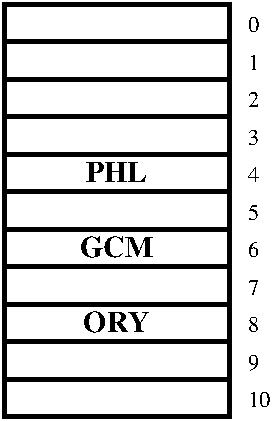
\includegraphics[height=0.33333\textheight]{../Images/hashapt.pdf}
\end{center}
\item However, inserting "HKG" causes a collision.
\begin{center}
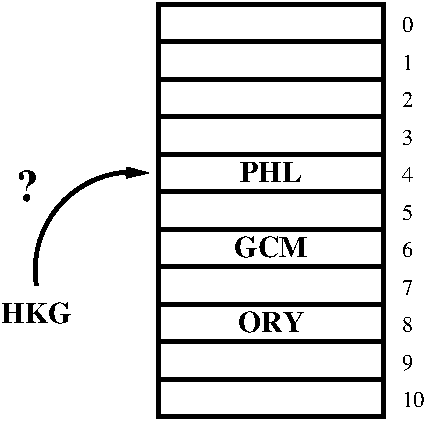
\includegraphics[height=0.33333\textheight]{../Images/hashclash.pdf}
\end{center}
\end{itemize}
\end{column}

\end{columns}
\end{frame}

%%%%%%%%%%%%%%%%%%%%%%%%%%%%%%%%%%%%%%%%%%%%%%%%%%%%%%%%%%%%%%

\begin{frame}[fragile]
\frametitle{Hashing : Collisions}
\begin{columns}[T]

\begin{column}{0.45\textwidth}
\begin{itemize}[<+->]
\item An ideal hashing function maps keys into the array in a {\it uniform} and {\it random} manner.
\item Collisions occur when a hash function maps two different keys onto the same address.
\item It's very difficult to choose `good' hashing functions.
\item Collisions are common - the {\bf von Mises} paradox. When 23 keys are randomly mapped onto 365 addresses there is a 50\% chance of a collision.
\end{itemize}
\end{column}

\pause
\begin{column}{0.45\textwidth}
\begin{itemize}[<+->]
\item The policy of finding another free location if a collision occurs is called open-addressing.
\item If a collision occurs then keep stepping backwards (with wrap-around) until a free location is encountered.
\pause
\begin{center}
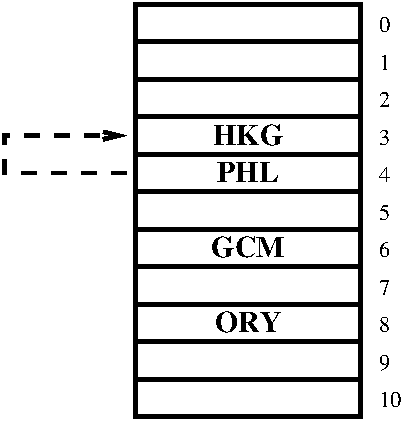
\includegraphics[height=0.3333\textheight]{../Images/hashprobe.pdf}
\end{center}
\end{itemize}
\end{column}

\end{columns}
\end{frame}

%%%%%%%%%%%%%%%%%%%%%%%%%%%%%%%%%%%%%%%%%%%%%%%%%%%%%%%%%%%%%%

\begin{frame}[fragile]
\frametitle{Double Hashing}
\begin{columns}[T]

\begin{column}{0.35\textwidth}
\begin{itemize}[<+->]
\item This simple method of open-addressing is linear-probing.
\item The step taken each time (probe decrement) need not be~1.
\item Open-addressing through use of linear-probing is a very simple technique, double-hashing is generally much more successful.
\item A second function p(K) decides the size of the probe decrement.
\end{itemize}
\end{column}

\pause
\begin{column}{0.55\textwidth}
\begin{itemize}[<+->]
\item The function is chosen so that two keys which collide at the same address will have different probe decrements, e.g. :
{\small
\[
p(K) = MAX (1, ((X_2*26^2 + X_1*26+X_0)/11)\%11)
\]
}
\item Although "PHL" and "HKG" share the same primary hash value of $h(K)=4$, they
have different probe decrements:

$p("PHL")=4$\\

$p("HKG")=3$
\end{itemize}
\end{column}

\end{columns}
\end{frame}

%%%%%%%%%%%%%%%%%%%%%%%%%%%%%%%%%%%%%%%%%%%%%%%%%%%%%%%%%%%%%%

\begin{frame}[fragile]
\frametitle{Hashing : Primes and Chaining}
\begin{columns}[T]

\begin{column}{0.45\textwidth}
\begin{itemize}[<+->]
\item If the size of our array, $M$, was even and the probe decrement was chosen to be $2$, then only half of the locations could be probed.
\begin{center}
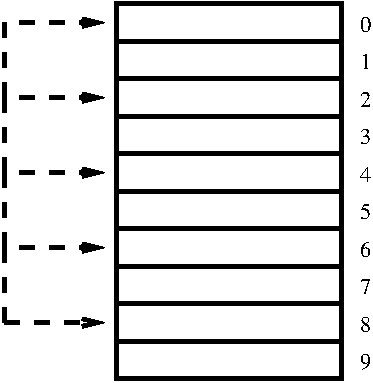
\includegraphics[height=0.4\textheight]{../Images/hashp2.pdf}
\end{center}
\item Often we choose our table size to be a prime number and our probe decrement to be a number in the range $1 \ldots M-1$.
\end{itemize}
\end{column}

\pause
\begin{column}{0.45\textwidth}
Open-addressing is not the only method of collision reduction. Another common
one is separate chaining.
\begin{center}
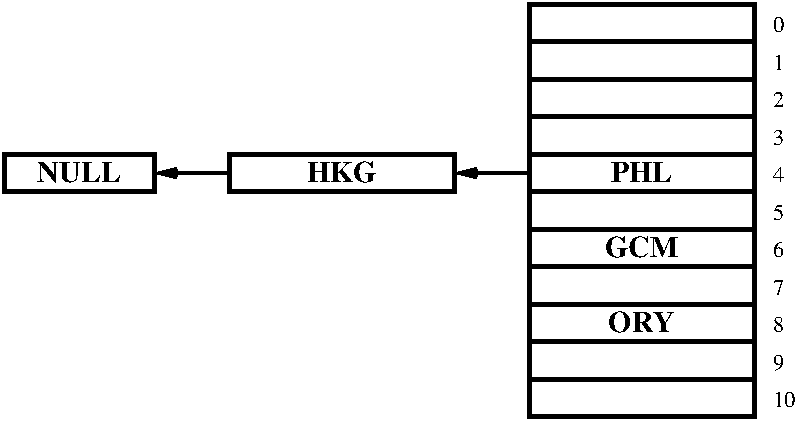
\includegraphics[width=1.0\textwidth]{../Images/hashsep.pdf}
\end{center}
\end{column}

\end{columns}
\end{frame}

%%%%%%%%%%%%%%%%%%%%%%%%%%%%%%%%%%%%%%%%%%%%%%%%%%%%%%%%%%%%%%

\begin{frame}[fragile]
\frametitle{A Practical Hash Function}
\begin{columns}[T]

\begin{column}{0.45\textwidth}
\lstinputlisting[style=basicc]{../Code/ChapU/bernstein.c}
\outputlisting{../Code/ChapU/bernstein.autoout}
\end{column}

\pause
\begin{column}{0.45\textwidth}
{\small
Has similarities to the implementation of \verb^rand()^~:
}
\lstinputlisting[style=basicc,linerange={22-46},numbers=none]{../Code/ChapU/rand.c}
\outputlisting{../Code/ChapU/rand.autoout}
\end{column}

\end{columns}
\end{frame}


%%%%%%%%%%%%%%%%%%%%%%%%%%%%%%%%%%%%%%%%%%%%%%%%%%%%%%%%%%%%%%

\begin{frame}[fragile]
\frametitle{Cuckoo Hashing}
\begin{columns}[T]

\begin{column}{0.45\textwidth}
\begin{itemize}[<+->]
\item We have two tables, each with their {\bf own} hash function.
\item We only need to check two cells when searching.
\item On collision, the existing item is `cuckooed' out of it's cell into the other table.
\end{itemize}
{\tiny
\begin{verbatim}
Empty: copied farandoles into table 0(4)
Empty: copied bronzine into table 0(12)
Empty: copied auscultatory into table 0(5)
Empty: copied bifer into table 0(13)
Empty: copied steepgrass into table 0(6)
Empty: copied prevised into table 0(7)
Empty: copied oomph into table 0(8)
empodium, so cuckooed out auscultatory from table 0(5)
Empty: copied auscultatory into table 1(10)
interquarreled, so cuckooed out bronzine from table 0(12)
Empty: copied bronzine into table 1(5)
ranseur, so cuckooed out empodium from table 0(5)
Empty: copied empodium into table 1(4)
Empty: copied megalodon into table 0(11)
geosynchronous, so cuckooed out megalodon from table 0(11)
Empty: copied megalodon into table 1(14)
Empty: copied osmeteria into table 0(14)
Table getting full -> rehashed old sz =16
\end{verbatim}
}
\end{column}

\pause
\begin{column}{0.45\textwidth}
\begin{center}
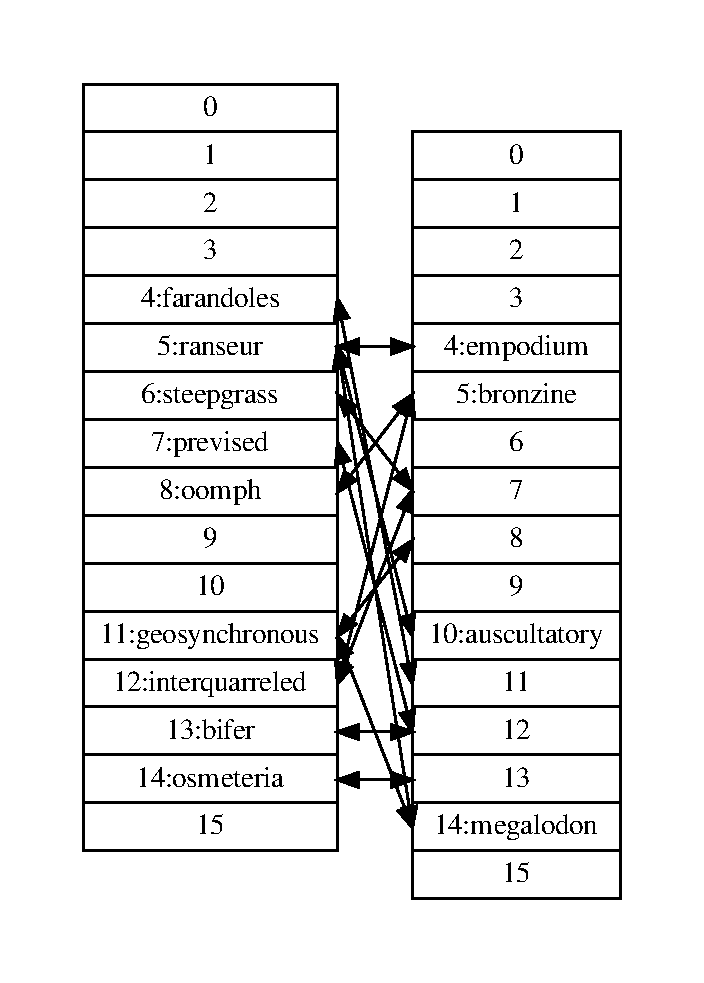
\includegraphics[height=0.8\textheight]{../Images/cuckoo.pdf}
\end{center}
\end{column}

\end{columns}
\end{frame}

%%%%%%%%%%%%%%%%%%%%%%%%%%%%%%%%%%%%%%%%%%%%%%%%%%%%%%%%%%%%%%
\endinput 
